\documentclass[a4paper,12pt]{article}
\usepackage[left=3cm,right=2.5cm,top=2.5cm, bottom=2.5cm]{geometry} 
\usepackage[utf8]{inputenc}
\usepackage{t1enc}
\usepackage{graphicx}
\usepackage[magyar]{babel}
\usepackage[nottoc]{tocbibind}%hogy az irodalomjegyzék is benne legyen a tartalomjegyzékben
\usepackage{pdfpages}

\usepackage{commath} %abszolút érték jelhez.
\usepackage{multirow}
\usepackage{subcaption}
\usepackage{subfig}



%matgót megoldottam a 2. sorban.
%\usepackage{anysize} %margóhoz
%\marginsize{3cm}{3cm}{2.5cm}{2.5cm}


%ha esetleg ki akarod szerni az összes ábrát ->
%\usepackage{comment}
%\excludecomment{textcolor}
%\excludecomment{figure}
%\let\endfigure\relax
%<-
\linespread{1.3} %1.3 = másfélszeres sorköz.
%\usepackage{showframe} -> megjelnnek a margók.

\begin{document}
\frenchspacing
%%%%%%%%%%%%%%%%%%%%%%%%%%%%%%%%%%%%%%%%%%%%%%%%%%%%%%%%%%%%%%%%%


\pagenumbering{gobble}

 \begin{center} 
\includegraphics[width=80mm,keepaspectratio]{abrak/bmelogo.jpg}\\ \vspace{0.3cm}  \Large Diplomamunka \\[1.5cm] \vspace{0.5cm} { \large \textbf{ Mikro-CT készülék rekonstrukciós és kalibrációs környezetének létrehozása}}\\[2.5cm] \vspace{0.2cm} \large Marinovszki Árpád\\[5cm] \begin{tabular}{ll} Témavezető: & Dr.\ Légrády Dávid \\ & egyetemi docens \\ & BME Nukleáris technika Intézet \\ \end{tabular} \vfill \large BME \\ \large 2016 \end{center} 
 
 \clearpage \setcounter{page}{1}
 \pagenumbering{arabic}
 
   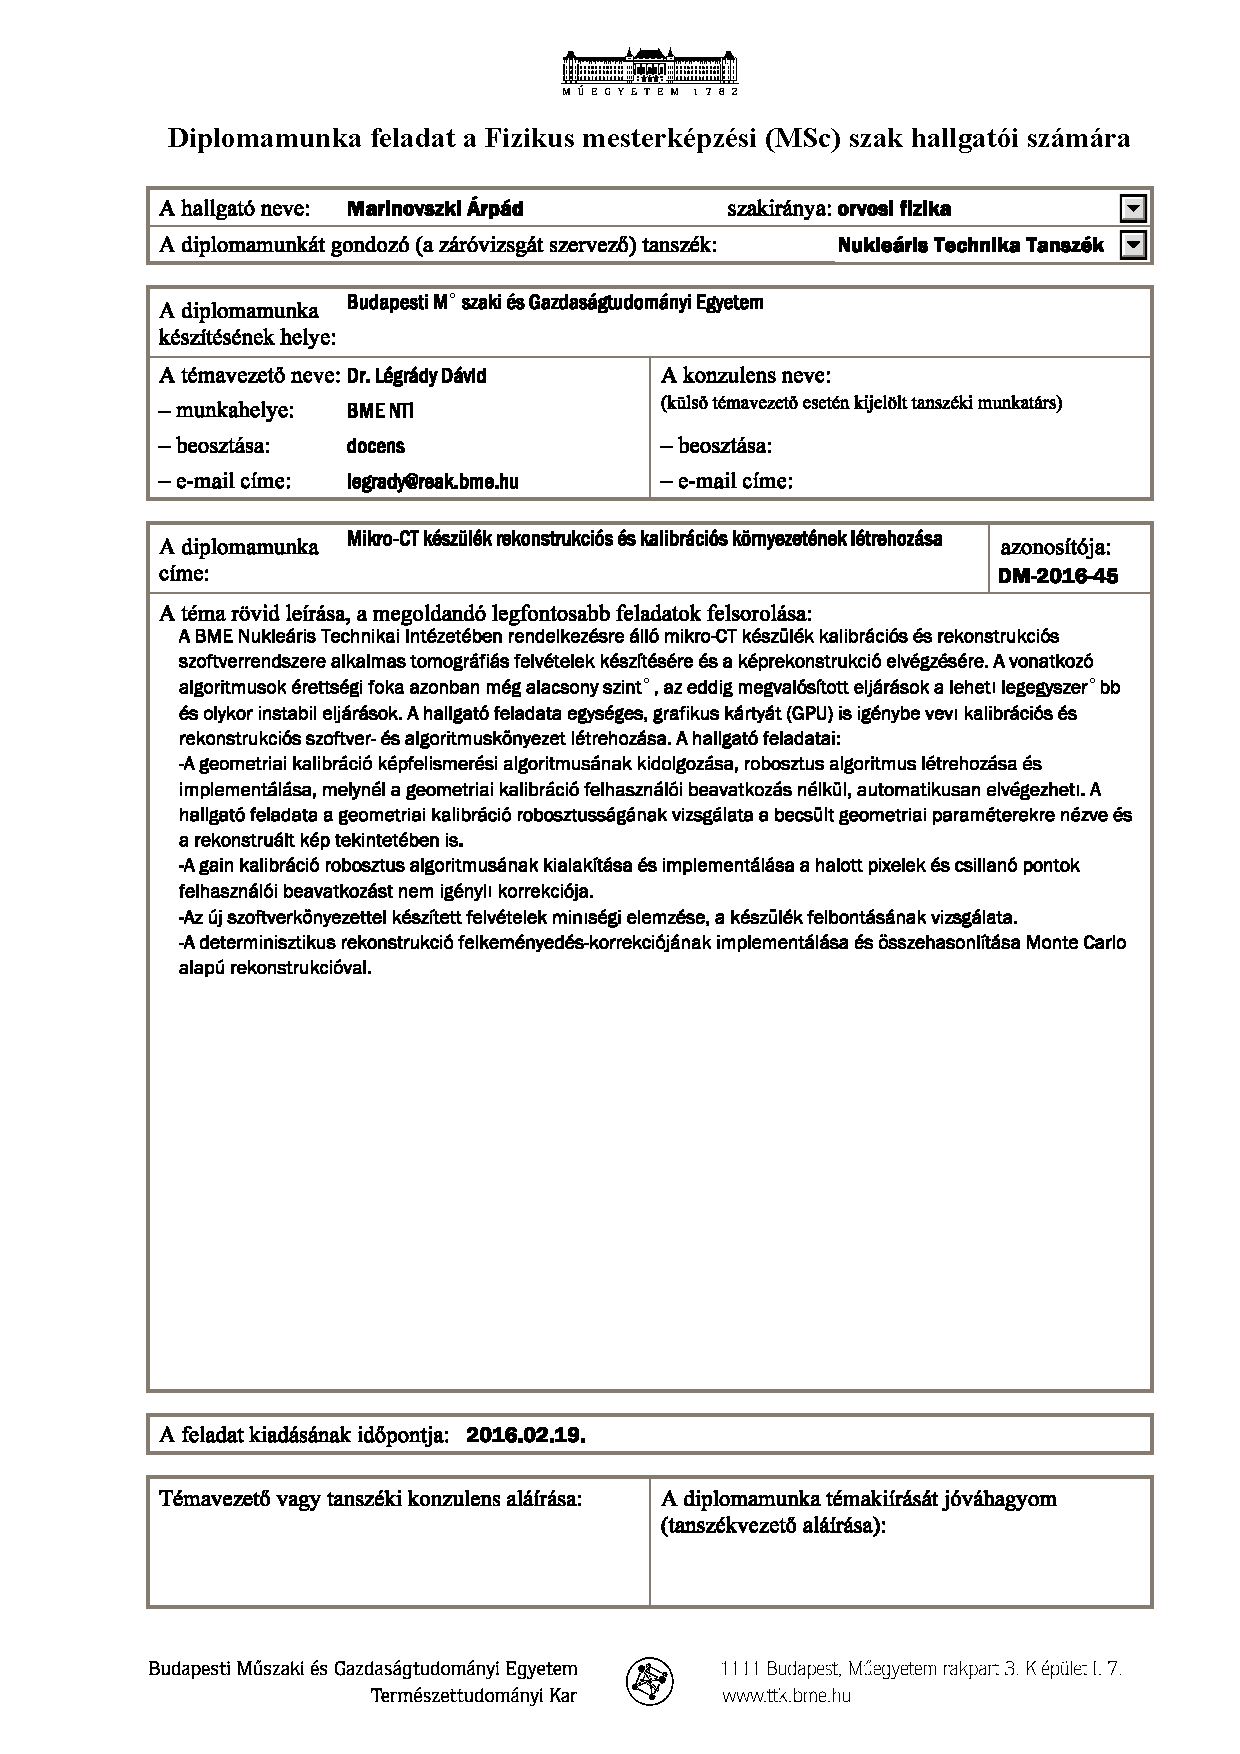
\includepdf[ pagecommand={}]{abrak/jelentkezes.pdf}

\clearpage

{\large Önállósági nyilatkozat}
\\[0.5cm]



Alulírott Marinovszki Árpád a Budapesti Műszaki és Gazdaságtudományi Egyetem fizikus MSc szakos hallgatója kijelentem, hogy ezt a diplomamunkát meg nem engedett segédeszközök nélkül, önállóan, a témavezető irányításával készítettem, és csak a megadott forrásokat használtam fel. 


Minden olyan részt, melyet szó szerint, vagy azonos értelemben, de átfogalmazva más forrásból vettem, a forrás megadásával jelöltem.
\\[0.3cm]

Budapest, 2016.\ június 6.

\hspace{9cm}\makebox[1.5in]{\hrulefill}

\hspace{9cm}\makebox[1.5in]{\centering aláírás}




\clearpage


 \tableofcontents

\clearpage

	






%CSAPJUNK A LECSÓBA
%TODO majd egyeztesd az egyes fejezeteken belül a személyeket és az igeidőt (csináljuk / csinálják/ csinálták stb)
%BEVEZETÉS------------------------------------------------------
\section{Bevezetés}

\section{Gain korrekció}


A gain korrekció az elkészült felvételeken elsődlegesen elvégzendő korrekció, amely felelős egyrészt azért, hogy a detektorpixelek eltérő érzékenysége és zaja következtében fellépő képhibákat eltüntesse. Továbbá, hogy korrigálja a röntgennyaláb mért intenzitásában történő azon gyengülést, amely pusztán azért következik be, mert a detektorpixelek más--más távolságra vannak a forrástól.

A fejezet elején megmutatom, hogy milyen hibákat eredményez a gain korrekció elhanyagolása. Ez után ismertetem a korrekció elvégzéséhez szükséges algoritmusokat és méréseket, majd bemutatom, hogy implementáltam a gain korrekciót az elkészült programban. 

\subsection{A gain korrekció által javított artefaktumok bemutatása}

A gain korrekció által kiszűrt hibák három részre oszthatóak. Egyrészt belátható, hogy a sík detektoron egy pontszerű forrásból származó fluxus értéke nem egyenletes. Ha olyan felvételt tekintünk, ahol nincs leképezendő objektum, a legnagyobb fluxus a detektor azon pixelét fogja érni, amely a legközelebb van a röntgenforrás fókuszpontjához. Az ettől távolabbi pixeleken mérhető intenzitás pusztán azért is kisebb lesz, mert a forrásponttól távolabb vannak, hiszen a mérhető intenzitás a fókuszponttól számított távolság négyzetének inverzével arányos. A jelenség következtében tehát a detektorpixelek intenzitása a detektor szélei felé csökken, és a csökkenés mértéke az expozíciós beállításoktól -- úgy mint az expozíciós idő, valamint a röntgencső feszültsége és árama -- független. A kialakult képtorzulást \emph{flatness hibának} nevezzük, utalva arra, hogy ez azért következik be, mert a detektorunk sík -- gömbfelületű detektornál ez a hiba nem lépne fel.

Megállapítható továbbá, hogy a detektorpixelek eltérő érzékenysége miatt is fellépnek képhibák. Ezen hibákat két csoportra lehet bontani: \emph{offset hibára}, valamint \emph{gain hibára}. Az elnevezés igen szemléletes, amelynek megértéséhez a következőket kell végig gondolnunk. 

Válasszunk ki a detektoron egy adott pixelt, és vizsgáljuk ennek a pixelnek az mért intenzitását, miközben változtatjuk az expozíciós időt! Az adott pixelen a mért intenzitás -- expozíciós idő függvényt ábrázolva olyan görbét kapunk, amely kezdetben igen jó közelítéssel egyenest mutat, mígnem az intenzitás egy adott értéket elérve nem nő tovább. Utóbbi esetet, azaz, amikor az intenzitásérték tovább nem nő, szaturációnak hívjuk. Ez a jelenség a hobbifotózásból is ismeretes: a detektor a ráeső fluxus egy adott tartományához rendel hozzá egy -- jelen esetben egész -- számot, mint intenzitás értéket. Amennyiben a maximális értékez tartozó fluxusnál nagyobb éri a detektort, akkor az továbbra is a lehető legnagyobb intenzitásértéket fogja kimenetül szolgáltatni, ekkor már a valós fluxus nagyságától függetlenül. 

Az előbbihez hasonlóan, ha állandó expozíciós idő mellett a röntgencső áramerősségét változtatjuk, és így nem a felvétel idejét növeljük, hanem a detektorra eső nyalábintenzitást, szintén kezdetben lineáris, majd telítődő összefüggést kapunk a pixel által mért intenzitás -- alkalmazott áramerősség függvény tekintetében. Éppen ezért az expozíciós idő és a röntgencső áramerősségének szorzatának -- a továbbiakban \emph{expozíció} függvényében szokás vizsgálni az adott pixel intenzitását. Az így kapott görbe, azaz az intenzitás az expozíció függvényében, adja meg az adott pixel érzékenységét.

Ez az érzékenység azonban pixelről pixelre változik. Különböző pixelek érzékenységét megvizsgálva észrevehetjük, hogy az egyes érzékenységi görbék lineáris szakaszának meredeksége és tengelymetszete is változik. Változik továbbá a szaturációs expozíció is, azaz az az expozíció érték, amelynél az adott detektor telítésbe megy. Ezt szemlélteti \aref{fig:gaingrafikon}.~ábra, amelyen négy különböző pixel által mért intenzitást ábrázoltam, az expozíció függvényében. Az ábrán jól látszódik, hogy a különböző pixelek érzékenysége eltérő meredekségű és tengelymetszetű egyenessel jellemezhető, valamint a szaturációs expozíciójuk is eltérő. Az offset és gain korrekciók a detektorpixelek ezen érzékenységbeli különbségeit korrigálják. A \emph{gain hibák} javítása jelenti az érzékenységek lineáris szakaszainak eltérő meredekségéből, tengelymetszetéből, valamint az eltérő szaturációs expozíciókból származó hibák javítását. Ezek tehát az expozíciós beállításoktól függő hibák.
Az \emph{offset hibák} javítása jelenti a mérés során a háttérből -- tehát nem a méréshez szükséges röntgen forrásból -- , valamint a zajokból származó mért intenzitásokat.  Az offset  hibák nagysága nem függ tehát az expozíciótól, de függ az expozíciós időtől. Ugyanis kikapcsolt röntgenforrás mellett is detektálunk valamekkora háttérsugárzást, illetve a detektorok zaja is mérhető intenzitást fog eredményezni a felvételen. A teljes, röntgenforrás nélkül mért jel arányos lesz az expozíciós idővel, hiszen minél tovább mérjük a detektor zaját, az annál nagyobb értéket fog képviselni. Továbbá a mért háttér függ a pixelek érzékenységétől is: egy jobban erősítő pixel a zajt is jobban erősíti. Az offset hibákat  tehát a pixelenkénti mért intenzitás -- expozíciós idő görbét felvéve tudjuk javítani.





\begin{figure}[htbp]
\center
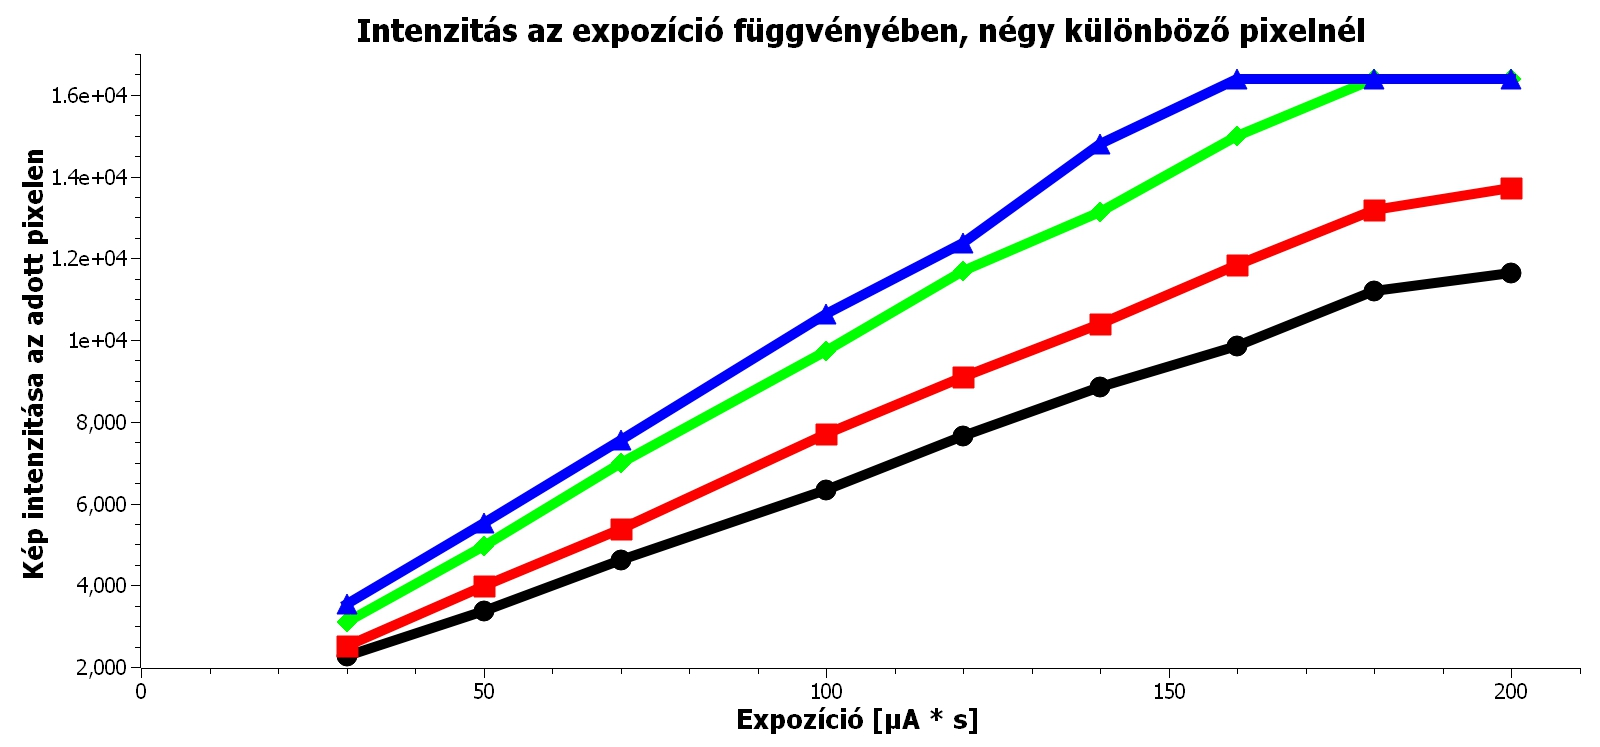
\includegraphics[width=0.8\textwidth]{abrak/gaingrafikon}
\caption{Négy kiszemelt pixel intenzitásának változása az expozíció függvényében.}
\label{fig:gaingrafikon}
\end{figure}




Az egyes hibák hatását az elkészült felvételeken \aref{fig:gainnelkul}.~ábrán szemléltetem. Az ábrán egy olyan felvétel látható, amely készítésekor a detektor és a forrás között leképezendő objektum nem volt, továbbá a felvétel mindenféle korrekciótól mentes, azaz a mérőszoftver ezt a képet olvasta ki a detektorból. Az ábrán látható, hogy a leképezendő objektum hiányában homogénnek várt kép közel sem homogén. Általánosan megfigyelhető, hogy az egyes pixelek értékei jócskán szórnak, továbbá látható, hogy a képen négyzetrácsos struktúra rajzolódik ki, amelynek oka  az, hogy detektorpanelek határainál megváltozik a pixelek érzékenysége. Különösen határozott ez az eltérés a képen látható hat függőleges egyenes mentén. Ezen pixelek az összes felvételen alacsonyabb intenzitással rendelkeznek társaiknál és értékük is kevésbé változik az expozíció növelésével, mint a többi pixel. Megfigyelhető továbbá, hogy a kép egyre sötétebb a sarkok felé, amely a flatness hibáak tudható be.

\begin{figure}[htbp]
\center
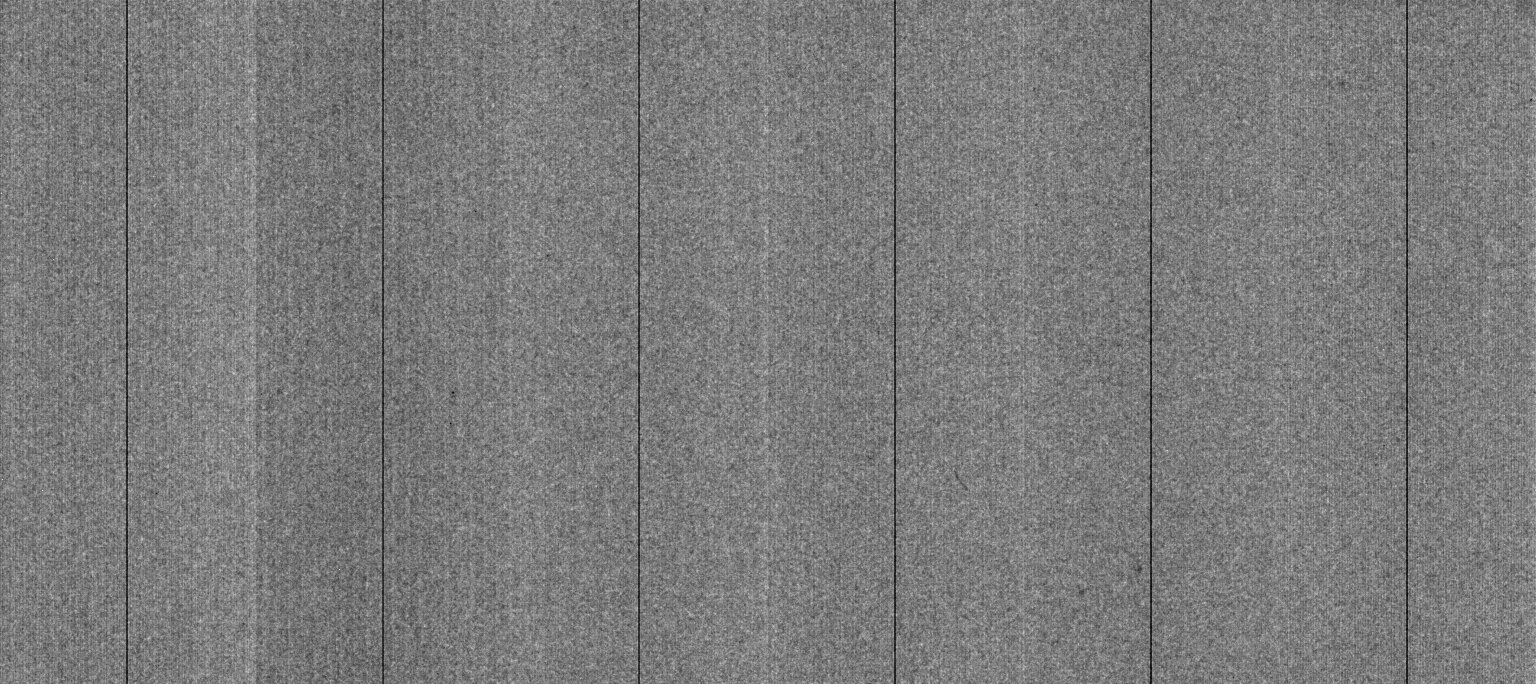
\includegraphics[width=1.0\textwidth]{abrak/gainnelkul}
\caption{Tárgy nélkül készített felvétel, gain korrigálás nélkül.}
\label{fig:gainnelkul}
\end{figure}

A gain korrekció során tehát ezen hibákat távolítjuk el a képről. Gain korrekció után a fenti képből \aref{fig:gainnel}.~ábrán látható képet kapjuk. Megfigyelhetjük, hogy itt nem látszódnak az előbb jelölt artefaktumok. Bár a kép továbbra sem teljesen homogén -- ezt nem is várjuk el, valamekkora zaj mindenképp terhelni fogja a méréseinket --, a pixelek intenzitásának szórása jóval lecsökkent, megszűnt a gain korrekció nélküli képet átható négyzetes struktúra, és a kevésbé érzékeny pixelek sem lógnak ki a többi közül. A következőkben ezen  gain korrekcióhoz szükséges algoritmusokat ismertetem.

\begin{figure}[htbp]
\center
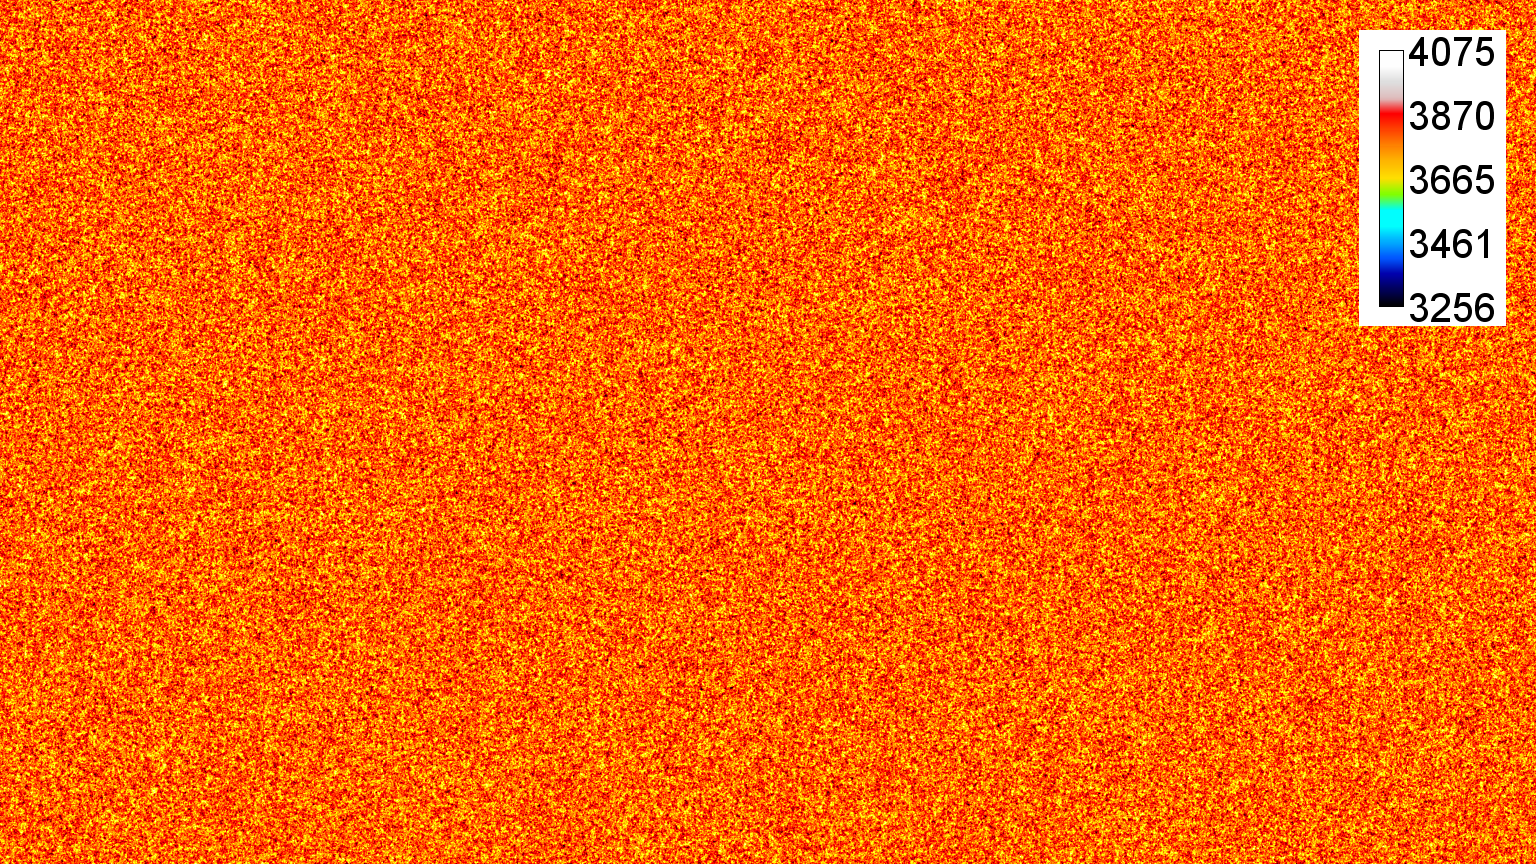
\includegraphics[width=1.0\textwidth]{abrak/gainnel}
\caption{Tárgy nélkül készített felvétel, gain korrigálás után.}
\label{fig:gainnel}
\end{figure}

\subsection{A gain korrekció algoritmusai}

A felvételek gain korrigálásához először is meg kell határozni az egyes detektorpixelekhez tartozó érzékenységeket, azaz azt, hogy az expozíció növelésével milyen gyorsan változik a pixel intenzitása, valamint azt, hogy az adott pixel milyen expozíció melett telítődik. ezen kívül meg kell határozni, hogy megvilágítás nélkül hogyan változik az adott pixel intenzitása az expozíciós idő függvényében. Ehhez először kalibráló képsorokat kell készíteni. Az offset hibák javításához a röntgenforrás bekapcsolása nélkül, különböző expozíciós időkkel, a gain és flatness hibák javításához bekapcsolt forrással, különböző expozíció értékek mellett. 

A képeket először az offset hibáktól kell megszabadítani, mivel azok a leképezendő objektumtól és a forrás beállításaitól függetlenül vannak jelen. Az ehhez szükséges korrekciós faktorok meghatározásához tehát különböző expozíciós időkkel, kikapcsolt forrással készítünk képeket. Az egyes pixelek értékét az expozíció idő függvényében ábrázolva olyan görbét kapunk, amelyre jól illeszthető egyenes. Ez alapján az $i$. pixel által, forrás nélkül mért $ I_i^{\text{offset}}$ intenzitás \aref({eq:offset}) képlettel írható le, ahol $a_i^{\text{offset}} $ és $b_i^{\text{offset}}$ a fenti módon előállított képsorozatból, egyenes illesztéssel megkapható és pixelenként változó paraméterek.

\begin{equation}
\label{eq:offset}
I_i^{\text{offset}} =  a_i^{\text{offset}} \cdot t_{\text{exp}} + b_i^{\text{offset}}
\end{equation}

Az offset hibák korrigálása után  az $i$. pixel intenzitása \aref({eq:offsetkorr})~ képlet szerint alakul, ahol $I_i^{\text{mért}}$ az $i.$ pixel eredeti, korrekció nélküli intenzitása, $I_i^{\text{offsetkorrigált}}$ pedig az offset hibától mentes érték.

\begin{equation}
\label{eq:offsetkorr}
\begin{split}
I_i^{\text{offsetkorrigált}}  &=  I_i^{\text{mért}} - I_i^{\text{offset}} \\&=  I_i^{\text{mért}} - \left( a_i^{\text{offset}} \cdot t_{\text{exp}} + b_i^{\text{offset}} \right)
\end{split}
\end{equation}


Ez után javíthatjuk ki a gain és flatness hibákat. A két hiba valójában egy algoritmussal javítható, hiszen a flatness hiba felfogható úgy, mintha a detektor pixeleinek érzékenysége lenne más a detektor más--más területein. A szükséges korrekciós faktorok meghatározásához olyan kalibráló képsorokat kell készítenünk, amelyek különböző expozícióval készülnek. \Aref{fig:gaingrafikon}.~ábrán látottak alapján megállapítható, hogy az egyes detektorpixelek intenzitása kezdetben az expozícióval lineárisan változik, vagyis egyenest tudunk rá illeszteni. Amennyiben tehát nincs tárgy a detektor és a forrás között, az $i$. pixel által, a detektort érő sugárzás, mint hasznos jel által okozott ( tehát offset hibától mentes) $ I_i^{\text{offsetkorrigált}}$  intenzitás értéke \aref({eq:gain})~egyenlet szerint számolható az expozícióból. Itt $a_i^{\text{gain}}  $ és $b_i^{\text{gain}}$ jelöli a különböző expozíciós értékek mentén felvett intenzitásértékekre illesztett egyenes paramétereit, $E$ pedig az expozíció értékét, amely a fent leírtak alapján az expozíciós idő és a röntgencső áramának szorzata.

\begin{equation}
\label{eq:gain}
\begin{split}
I_i^{\text{offsetkorrigált}}  &=  I_i^{\text{mért}} - I_i^{\text{offset}} \\&=  a_i^{\text{gain}} \cdot E + b_i^{\text{gain}}
\end{split}
\end{equation}

Egy olyan felvételen, amely készítésekor valamilyen tárgyat helyezünk a detektor és a forrás közé, a mért intenzitásértékek nyilván el fognak térni a detektor különböző részein, ahogy a leképezni kívánt tárgy lineáris gyengítési együtthatója is eltér a különböző térfogatokban. Ezt úgy vehetjük figyelembe, hogy  \aref({eq:gain})~képletben az $E$ expozíció érték helyére egy helyfüggő, $E_i^{\text{virt}}$ virtuális expozíciót vezetünk be. Ezen érték úgy módosul az eredeti $E$ expozícióhoz képest, hogy figyelembe veszi a röntgen nyaláb gyengülését, miközben az áthalad a leképezni kívánt tárgyon. Vagyis egy adott mérés során az $E_i^{\text{virt}}$ virtuális expozíció nem lesz más, mint az a (valós) expozíció érték, amely esetén ugyan akkora intenzitást mértünk volna tárgy nélküli elrendezésben, mint jelen esetben a leképezendő tárggyal. Ezzel a jelöléssel kapjuk \aref({eq:gain_virtual}) egyenletet, amely immáron általánosan igaz, egy tetszőleges felvételre -- míg \aref({eq:gain})~egyenlet csak arra az esetre érvényes, amikor nincs semmi a detektor és a forrás között.

\begin{equation}
\label{eq:gain_virtual}
\begin{split}
I_i^{\text{offsetkorrigált}}  &=  I_i^{\text{mért}} - I_i^{\text{offset}} \\&=  a_i^{\text{gain}} \cdot E_i^{\text{virt}} + b_i^{\text{gain}}
\end{split}
\end{equation}


A gain hibák javítása során azt szeretnénk elérni, hogy az egyes pixelek intenzitása ne függjön az adott pixel érzékenységétől, azaz az $a_i^{\text{gain}}  $ és $b_i^{\text{gain}}$  együtthatóktól, csak az adott pixelt ért -- virtuális -- expozíciótól. Vagyis azt, hogy ha két detektorpixelt egy felvétel során ugyanolyan intenzitású sugárzás ér, és az expozíciós idő is megegyezik, akkor a két pixel intenzitása az elkészült képen is azonos legyen. 
Ezt úgy végezzük el, hogy először meghatározzuk az egyes detektorpixelek virtuális expozícióját, majd ezekből úgy alakítjuk ki a gain korrigált intenzitásértéket, mintha minden pixel érzékenysége megegyezne.

Először tehát kiszámoljuk az adott offset korrigált intenzitáshoz tartozó virtuális expozíció értékét \aref({eq:gain_virtual})~egyenlet segítségével, amelyből egyszerű átrendezéssel kapjuk a virtuális expozícióra  \aref({eq:virtual_expozicio})~egyenletet. 

\begin{equation}
\label{eq:virtual_expozicio}
\begin{split}
 E_i^{\text{virt}} &= \frac{I_i^{\text{offsetkorrigált}} -  b_i^{\text{gain}}}{  a_i^{\text{gain}}}
 \end{split}
\end{equation}



 A virtuális expozíció tehát azzal van összefüggésben, hogy mekkora valós fluxus érte az adott pixelt, és mentes az adott pixel érzékenységek torzító hatásától. Ebből úgy határozzuk meg a gain korrigált intenzitás értéket, mintha minden pixel érzékenysége, azaz intenzitás -- virtuális expozíció függvénye egy origón átmenő egyenes lenne, mindnek azonos meredekséggel. A szóban forgó meredekséget pedig úgy határozzuk meg, hogy éppen annál az expozíciós értéknél telítődjön, amelynél a legérzékenyebb pixel már telítődik. Azaz meg kell vizsgálni, hogy az expozíciót növelve mikor kapunk olyan képet, amin már van szaturált pixel. Ezen expozíciót hívjuk szaturációs expozíciónak ($E^\text{szat}$). Ezen érték a kalibráló adatsorból szintén meghatározható paraméter. Ezen paraméter ismeretében a gain korrigált $ I_i^{\text{gainkorrigalt}}$ pixelintenzitás \aref({eq:gainkorrigalt})~egyenlettel számolható, ahol $\left(2^{14} -1\right)$ a detektor által mérhető maximális intenzitásérték.

\begin{equation}
\label{eq:gainkorrigalt}
\begin{split}
 I_i^{\text{gainkorrigalt}} &= E_i^{\text{virt}}  \cdot \frac{2^{14} -1}{E^\text{szat}}
 \end{split}
\end{equation}


A módszer hatékonyságát -- azaz azt, hogy a megfelelő adatsorokra valóban jól illeszkedik egyenes, valamint, hogy az így meghatározott korrekciós faktorokkal valóban hatékonyan lehet javítani a képek minőségét -- a kísérleti algoritmus létrehozása során Botond részletes tesztekkel vizsgálta, ezért én ettől eltekintek. Ugyanakkor megjegyzem, hogy a korrekciós faktorokat külön meg kell határozni minden feszültségértékre, amin a röntgenforrást működtetjük. A feszültség módosításával ugyanis megváltozik a detektorpixelekben a sugárzás elnyelődésének valószínűsége, azaz változik a pixel érzékenysége.


A továbbiakban azt mutatom be, hogy ezeket az algoritmusokat hogyan építettem bele az elkészült szoftverbe, illetve milyen mérési utasítást ajánlok a korrekciók elkészítéséhez.


\subsection{A gain kalibráció használata}


Mint ahogy már említettem  %TODO : említd is, a beveztésben
 a kalibrációs szoftver létrehozásakor szempont volt, hogy annak sebessége gyors, kezelése egyszerű legyen, így létrehoztam egy grafikus felülettel rendelkező programot, amelyben a felhasználó nyomógombokkal tud választani az elérhető funkciók között. Az első ilyen megvalósított funkció az offset és gain hibák korrigálására szolgáló együtthatók meghatározása. Ezt a funkciót választva a szoftver egy új ablakban kéri a felhasználót, hogy  válassza ki az elkészített kalibrációs mérések mappáját, valamint azt a mappát, ahova a kimeneti fájlokat menteni szeretné. Ez után a korrekciós faktorok számolása automatikusan megtörténik, minden olyan feszültségértékre, amely feszültség értékekkel megfelelő mennyiségű és minőségű kép található az adott mappastruktúrában (lásd alább). Az esetleges hibákról a felhasználó értesítést kap a konzolon.
 
 
 

A korrekciós faktorok  pixelenként kerülnek meghatározásra, így azok, mint egy együttható-térkép, képként  kerülnek mentésre.
 A diplomamunkához használt gain korrekciós faktorok 50kV-os feszültségen készült képekhez tartozó együttható térképét \aref({fig:offsetfaktorok}).~ és \aref({fig:offsetfaktorok2}).~ábrán láthatóak. A struktúrák jobb láthatósága érdekében az egyes képek ábrázolásához különböző színtérképeket használtam. Az ábrákon látjuk azt, hogy a detektor struktúrája valóban nagy hatással van az egyes pixelek érzékenységére. 
 
 
 \begin{figure}[htbp]
\center
\includegraphics[width=0.49\textwidth]{abrak/offsetslope}
\includegraphics[width=0.49\textwidth]{abrak/offsetintercept}
\caption{Offset hibák korrekciójára szolgáló együttható-térkép. Balra a korrekciós egyenes tengelymetszete, jobbra a meredeksége [ms$^{-1}$].}
\label{fig:offsetfaktorok}
\end{figure}

 
 
  \begin{figure}[htbp]
\center
\includegraphics[width=0.49\textwidth]{abrak/slope50}
\includegraphics[width=0.49\textwidth]{abrak/intercept50}
\caption{Gain és flatness hibák korrekciójára szolgáló együttható-térkép. Balra a korrekciós egyenes tengelymetszete, jobbra a meredeksége [($\mu$A $\cdot$ ms)$^{-1}$].}
\label{fig:offsetfaktorok2}
\end{figure}

 
 

 Ezekkel a korrekciós faktorokkal a felhasználónak lehetősége nyílik az elkészített projekcióit offset és gain korrigálni, az erre vonatkozó (\ref{eq:offsetkorr}) és (\ref{eq:gainkorrigalt}) képleteket felhasználva.  A felhasználónak ennél a funkciónál is grafikus felületen van lehetősége kijelölni a korrigálni kívánt mappát, amelyből a program az összes képet gain korrigálja és elmenti egy kívánt, kijelölt mappába -- akár ugyan abba. 
 
 
\subsection{A gain kalibráció implementálása és a szükséges mérések leírása} 
\label{sec:reduce}
 
 
A bemeneti fájlok elkészítéséhez, azaz a mérési utasításhoz szükséges megjegyeznem, hogy a mérések során észrevehető volt, hogy a detektor által készített képek egy része valamiért jóval sötétebb, mint az azonos körülmények között készült egyéb képek. Ez a hiba a képek kb.\ 5\%-át érinti, és okát nem sikerült felderíteni. Más felhasználók is panaszkodtak hasonló hibára ennél a detektortípusnál. A korrekciós faktorok számításánál azonban kimondottan fontos, hogy ilyen képeket ne használjunk fel a számításokhoz -- továbbá az ilyen képek kezelése egyéb helyzetekben is szükségszerűnek tűnik. Ennek érdekében a gain kalibrációhoz szükséges méréseket úgy végeztük el, hogy egy adott beállítással több képet készítettünk ( 10--20 képet beállításonként). Az azonos beállításokkal készült képeket külön mappákba mentettük, így a szoftver is ilyen formában várja azokat az adatok feldolgozása során. Ez a megoldás azért szerencsés, mert egy mappán belül átlagolva a képek intenzitásértékét, könnyen és egyértelműen kiszűrhető, ha valamelyik kép jóval sötétebb, a fent említett hiba miatt. Továbbá az azonos mappákban lévő, tehát azonos beállításokkal készült képeket átlagolva a képeket terhelő zaj is csökken. Így amikor a korrekciós faktorokat számolom, mappánként átlagolom azokat a képeket, amelyek átlagos intenzitása nem tér el 10\%-nál jobban a mappában lévő képek átlagos intenzitásának átlagától. Az program  robusztusságát  tovább növelve, a képek beolvasásakor vizsgálom, hogy  azok milyen expozíciós beállításokkal készültek, és ez alapján is szelektálom a képeket, kiszűrve a mérés során elkövetett emberi hibákat. A mérésvezérlő szoftverről ugyanis tudni érdemes, hogy a felvételek készítésének elindítása a röntgen forrás bekapcsolásától függetlenül elindítható, és az indítás után sorozatosan készít képeket, amíg le nem állítják. Mérés közben a forrás feszültsége és áramerőssége szabadon változtatható, illetve a forrás ki- és bekapcsolható. A röntgencső független kezelése részben biztonságvédelmi célokat szolgál, azonban lehetőséget ad a felhasználónak, hogy a képek sorozatos kimentését elindítsa úgy, hogy a forrás nincs bekapcsolva, vagy a beállított paraméterei nem megfelelők. Ekkor gyakran előfordul, hogy a felhasználó a paramétereket menet közben állítja, és az addigi eredményeket nem törli ki. Ezt kiküszöbölendő, a gain korrekcióhoz készített kalibrációs képek feldolgozása során a képek átlagos intenzitásán kívül a program vizsgálja az átlagos áramerősség, feszültség és exponálási idő paramétereket is, és a kilógó értékkel készült képeket figyelmen kívül hagyja. Továbbá figyelembe veszi azt is, hogy offset korrekcióhoz készült kalibráló képek között ne legyen olyan, ahol a forrás be volt kapcsolva -- vagy ha van, akkor hagyja azt is figyelmen kívül. Hasonlóan a gain és flattness hibák faktorai meghatározásánál az algoritmus ignorálja azokat a képeket, ahol a forrás ki volt kapcsolva. Amennyiben egy mappában kevés kép van, amely a fenti szűröknek megfelel (5-nél nem több), akkor a mappa tartalmát a szoftver nem használja fel a korrekciós faktorok meghatározásához. Továbbá, amennyiben túl kevés mappát talál a szoftver (5-nél nem többet), tehát túl kevés a különböző expozíciós beállítások száma a korrekciós faktorok meghatározásához -- akár összesen, akár túl kevés megy át a fenti szűrükön--, a kalibrációs  faktorok nem kerülnek meghatározásra. Így elkerülhető, hogy túl kevés pontra illesszünk egyenest, és ezért hibás eredményeket kapjunk, vagyis a képkészlet ellenőrzése szintén a szoftver robusztusságát növeli. A felvételek elkészítésekor alkalmazott feszültségértékeket az program szintén a képek beolvasásakor határozza meg, így azt külön megadni nem szükséges, mint ahogy a képeket feszültség szerint sem kell szétválogatni -- ellentétben a kísérleti algoritmussal.

A képek beolvasása és mappánkénti  átlagolása után a pixelenkénti egyenes illesztést a szokásos, egyenes illesztésére vonatkozó (\ref{eq:linearfit}) képleteket felhasználva oldottam meg, ahol az $x$ és $y$ mérési pontokra illesztjük az $\alpha$ és $\beta$ paraméterekkel jellemzett egyenest.  A képletben a felülvonás az átlagolást jelenti.

\begin{equation}
\label{eq:linearfit}
\begin{split}
\beta &= \frac{ \overline{xy} - \overline x \cdot \overline y }{\overline{x^2} - {\overline{x}}^2}\\
\alpha &= \overline y -\beta \cdot \overline x
\end{split}
\end{equation}


Jelen esetben $x$ értéke az expozíciós idő (offset hibáknál), vagy az expozíció (gain és flatness hibáknál), y pedig az adott pixel intenzitása. Az egyenes illesztésére egyszerű és gyors megoldásnak találtam, hogy az illeszteni kívánt képeket pixelemként összeadom, valamint ugyanezt megteszem az adott expozícióval -- vagy expozíciós idővel -- megszorozva is, majd ezeket a képeket pixelenként elosztom az összeadott képek számával. Így képek összeadásával és skalárral való osztásával az $\overline x$ és $\overline{xy}$ értékek pixelenként előállnak, mint egy--egy kép. Ez után a kettő különbségét -- mint képet -- leosztva az  $\left ( \overline{x^2} - {\overline{x}}^2\right )$ skalárral, közvetlenül előáll a pixelekre illesztett egyenes meredeksége, és a tengelymetszet további képkivonással kapható. Mivel a szükséges képműveletek -- összeadás, skalárral szorzás, kivonás -- könnyen párhuzamosíthatóak, gyakorlatilag az egyenes illesztése is párhuzamosan történik, így jelentősen lerövidítve a számoláshoz szükséges időt. 
%15 perc helyett 2 és fél perc. Az enyém átlagol mappánként, az övé nem.
 A módszer egyébként a memóriával is takarékosabban bánik, mint a kísérleti algoritmus, amely először beolvassa az összes képet a memóriába, majd pixelenként illeszt egyenest. Az ottani megoldással ellentétben, ahol a szükséges memória lineárisan nő a képek számával, nálam a szükséges memória a képek számától független és alacsony.


A fenti megoldáshoz a grafikus felületet és a mappakezelést a Qt biztosítja, míg a gyors képműveletek CUDA kód alkalmazásával valósulnak meg. A képfeldolgozáshoz létrehoztam olyan kép osztályt, amely képes magát fájlból a GPU memóriájába olvasni, és alkalmas a képeken végzett műveletek gyors végrehajtására a grafikus kártyán. A pixelenkénti összeadás, kivonás, skalárral szorzás megoldása viszonylag triviális, itt egy szál egy pixel értékét számolja. Ezzel ellenben a maximum, minimum és átlagos intenzitás számolása első ránézésre nem triviális, ezért néhány mondatban bemutatom. 

Az előbb felsorolt műveletek, amelyek eredménye előáll a kép pixeleiből úgy, hogy minden egyes pixel értékét egyszer használjuk fel, egy kommutatív, asszociatív, két elem között ható -- programozási értelemben vett -- operátorral, az angol irodalom  \emph{reduce} műveletnek hívja. Ilyen az előbb említett összeadás, minimum és maximum számítás is. Például három elem, $a,b$ és $c$ összegét megkapjuk, ha $a$ és $b$ összegéhez hozzáadjuk $c$-t: $\text{sum} = (a+b)+c$. Az összeadást kicserélhetjük maximum számításra is, az algoritmus ekkor csak a számok közé rakott operátorban tér el: $\text{maximum} = \text{max} ( \text{max}(a,b),c))$.  Az ilyen, \emph{reduce} típusú műveletek optimális használatát az összeadás példáján keresztül írom le, de a fentiek értelmében a minimum és a maximum számolás is hasonlóan kivitelezhető.

Az alkalmazásomban is használt reduce műveletet  a CUDA hivatalos dokumentációjához mellékelt példa \cite{reduce} alapján állítottam össze. Az ilyen műveletek általános megoldása -- az összeadás példáján --, hogy a képet két részre osztjuk, majd az egyik részt hozzáadjuk a másikhoz. A műveletet folytatjuk, mindig felezve a fennmaradó képrészletet, míg végül a kép egyik pixelében előáll az összes pixel összege. A már említett példa ezen túl olyan, CUDA specifikus technikákat is ajánl a művelet gyorsításához, mint a \emph{shared memory}, azaz az összes szál által hozzáférhető (de kívülről nem hozzáférhető), gyors elérésű memória használata -- a lassú elérésű, globális memória helyett, ahol a képek eleve tárolva vannak. Továbbá figyelembe veszi, hogy a párhuzamos futtatás során a szálak 32 darabos ,,csomagokban'',  úgynevezett \emph{warpokban} futnak, ezzel tovább optimalizálva az algoritmust. Abban az esetben ugyanis, ha több, mint 32 szálat futtatunk egyszerre, semmi nem garantálja, hogy azok egyszerre fognak futni. Ilyenkor időről időre be kell várnia a szálaknak egymást. Például ha a kép egyik felét hozzáadjuk a másikhoz, csak akkor felezhetjük tovább az elkészült képet, ha minden összeadás megtörtént. Amikor már 32-nél kevesebb szálat használunk, akkor a szálaknak nem kell egymást bevárni, hiszen biztosan nem fut több. Továbbá a példa alapján az összeadáshoz vonatkozó kerneleket C++ template-ekkel írtam meg, amely segítségével már fordítási időben tudja a kernel, hogy adott méretű kép esetén hogyan kell felosztani a képet -- nem pedig futási időben kell $if$ műveletekkel vizsgálnia, hogy a kép mekkora méretű. A hivatkozott példa alapján a \emph{reduce} műveletek ilyen technikákkal való megvalósítása akár $6$--$30$-szor gyorsabbak, mintha ezek nélkül valósítanánk meg a műveletet. Ez a program futási sebességére igen jótékony hatással van, hiszen a kép pixeleinek összeadására -- átlag számoláshoz -- szinte minden megnyitás után szükség van, hogy eldöntsük, hogy az az említett ismeretlen hiba miatt elsötétült e, vagy sem. 



%TODO A véletlenszerűen elsötétülő képeket itt is külön korrigálja a program: ha egy kép intenzitása jelentősen eltér a sorrendben mellette lévő képek átlagától, úgy az szoftvera képet a szomszédjainak átlagával helyettesíti a gain korigálás előtt.

\section{A geometria kalibráció}

A diplomaunkám során a másik megállapítandó kalibráció az úgynevezett \emph{geometria kalibráció}, amely a CT-vel elkészített képek alapján állapítja meg, hogy milyen távol van egymástól a detektor, a forgatható asztal forgástengelye és a röntgencső fókuszpontja. A geometriai adatokhoz igen pontosan szükség van, amikor az elkészült projekciók alapján meghatározzuk a felvett tárgy 3 dimenziós képét, vagyis a visszavetítéskor. Ugyanakkor a geometriai paramétereket kézzel nem tudjuk igen pontosan lemérni, már csak azért sem, mert a röntgencső fókuszpontjának a helye nem hozzáférhető és nem ismert, továbbá a mérési pontatlanság is viszonylag nagy lenne. Ezért alkalmazzuk azt a módszert, hogy az elkészült képek alapján határozzuk meg a szóban forgó paramétereket. 

A kalibrációt két cikk alapján végeztem el. Noo cikke\cite{noo} valamivel bonyolultabb  módon, kevés adatból határozza meg a geometriai paramétereket, míg Wu\cite{wu} cikke az előbbire támaszkodva, azonban azt leegyszerűsítve,  és több adatsorból határozza meg a távolságokat, a szerzők szerint pontosabban, mint a Noo féle megoldással. A kísérleti algoritmus ezért is csupán utóbbival dolgozik. Én azonban megvizsgáltam, hogy hibaszámítással alkalmazható e hatékonyan a Noo által leírt, kevesebb elhanyagolást tartalmazó módszer, valamint hibaszámítással javítottam a Wu által vázolt módszeren is, továbbá a kísérleti algoritmushoz képest fundamentálisan más megoldást vezettem be a képek feldolgozásához.

 A továbbiakban bemutatom a geometriai kalibráció meghatározásának elméletét a cikkek alapján, majd bemutatom, hogy a geometriai adatok meghatározásához milyen módszereket használt a kísérleti algoritmus, valamint az én algoritmusaim, továbbá ismeretem az elért eredményeimet. 

\subsection{A síkpaneles CBCT geometriája}

Hogy a geometriai kalibráció során milyen adatok kerülnek meghatározásra, és milyen adatok kerülnek elhanyagolásra, azt jól szemlélteti \aref({fig:geom1}).\ és \aref({fig:geom2}).~ábra. 



\begin{figure}[htbp]
\center
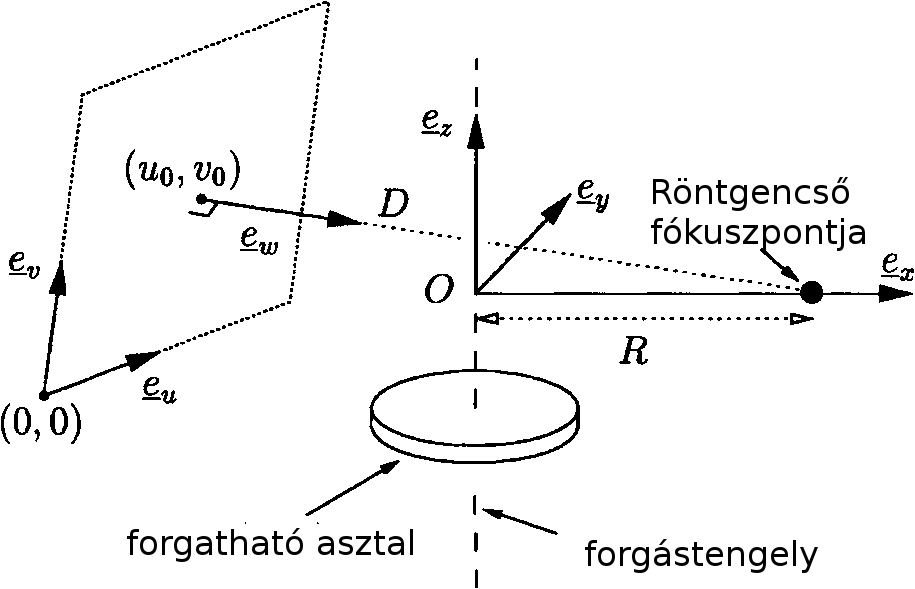
\includegraphics[width=0.5\textwidth]{abrak/geom1}
\caption{A Cone-beam CT elrendezésének vázlata\cite{noo}. A $z$ tengellyel párhuzamos forgástengely $R$ távolságra van az $x$ irányban lévő forrásponttól. A detektor és a forrás közötti legrövidebb távolság $D$. A forrásoz legközelebb eső pontja a detektornak az $u_0,v_0$ koordinátával jellemzett pixel. }
\label{fig:geom1}
\end{figure}





\Aref{fig:geom1}.~ábrán látható paraméterek jelentése a következő. A forgatható asztal forgástengelye és a röntgencső fókuszpontjának távolsága $R$. Konvenció szerint a forgástengely a $z$ tengellyel párhuzamos és az $x$ tengely irányában található a forrás fókuszpontja. A detektor az $(u_0,v_0)$ koordinátákkal jellemzett pixelétől mért távolsága a legkisebb a forrástól, és ez a távolság $D$.


\begin{figure}[htbp]
\center
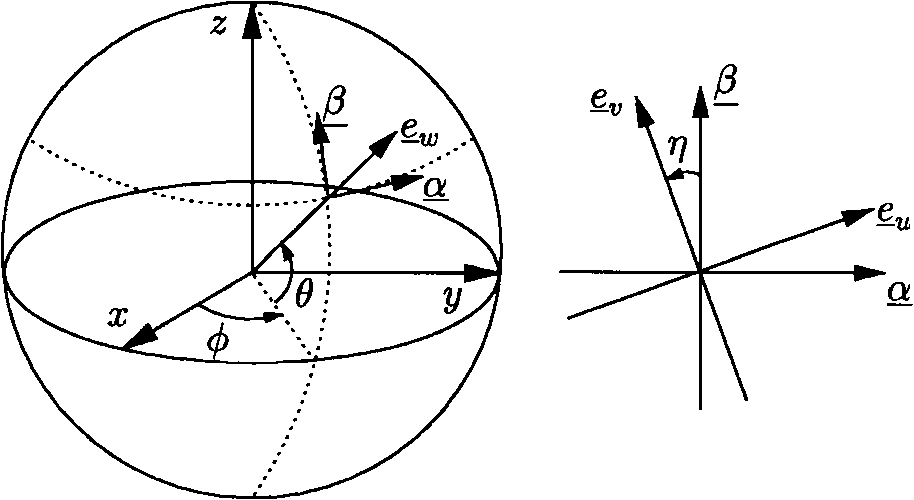
\includegraphics[width=0.5\textwidth]{abrak/geom2}
\caption{A Cone-beam CT elrendezésében jellemző irányok\cite{noo}. $\underline{e}_\omega$ a detektor síkjára merőleges irány, $\alpha$ és $\beta$ a detektor síkjában fekvő, egymásra merőleges vektorok. A detektor dőlését a $\phi, \theta,$ és $\eta$ szögek jellemzik.}
\label{fig:geom2}
\end{figure}



 \Aref{fig:geom2}.~ábrán azt láthatjuk, hogy míg a forgástengely és a forrás iránya  a modell szerint rögzített, a detektor irányát és állását a   $\phi, \theta$ és $\eta$ szögeket jellemzik. Ezek közül az $\eta$ szöget, vagyis a detektornak a saját síkjában való elfordulását mindkét cikk figyelembe veszi és számolja. A $\phi$ szöget, vagyis a detektor kifordulását, az asztal forgástengelyével párhuzamos tengely mentén, már csak Noo\cite{noo} cikke számolja ki. A $\theta$  szöggel jellemzett elfordulást pedig mindkét cikk elhanyagolja. Az elhanyagolásokra az ad lehetőséget, hogy az nem befolyásolja nagy mértékben a rekonstruált képeket, illetve a többi paraméter mérési pontosságát\cite{wu}. 

 Összefoglalva tehát meghatározandó paraméter a detektor és a forrás távolsága ($D$), a forgástengely és a forrás távolsága ($R$), a detektor pixelei közül a forráshoz legközelebbi ($u_0,v_0$), valamint a detektor elfordulása a saját síkjában ($\eta$).  Ezen kívül Noo módszerével meghatározható a detektor ferdeségét jellemző $\phi$ szög is, de ez egyrészt a kísérleti algoritmusban sem került meghatározásra, másrészt az elkészült rekonstrukciós kód sem veszi figyelembe.
 

\subsection{A geometriai paraméterek meghatározásának elmélete}

A fent összegzett paraméterek az említett cikkek alapján meghatározhatóak úgy, hogy a forgatható asztalra egy plexi --  vagy egyéb, alacsony sűrűségű -- lapra fém -- vagy egyéb, nagy sűrűségű -- gömb alakú tárgyakat helyezünk el, egymástól jól meghatározott távolságra, majd az asztalt körbeforgatva felvételeket készítünk. Belátható\cite{noo}, hogy a forgatás során körbeforduló gömbök a detektoron ellipszis pályát írnak le. A geometriai paramétereket ezen ellipszis pályákból tudjuk meghatározni.
Ennek módját először Noo cikke alapján mutatom be, majd ismertetem, hogy ahhoz képest Wu cikke milyen változásokat tartalmaz.

\subsubsection{A paraméterek meghatározása Noo\cite{noo} cikke alapján}
\label{sec:noo}


Az adatok feldolgozása mindkét esetben azzal kezdődik, hogy az egyes projekciókon meg kell keresni, hogy a detektoron hol jelenik meg a golyók képe. A sorrendben $k$.\ golyó helyzetét az $i$. projekción ($u_k^i, v_k^i$)-vel jelölöm. Noo cikkében két golyót tartalmazó fantomot használnak, így $k$ értéke 1 vagy 2 lehet. $i$ értéke 1 és $N$ között változik, ahol $N$ a teljes körbeforduláshoz alatt elkészített felvételek száma.  Az egyes projekción az említett koordináták megkeresése nem egyértelmű probléma, és az említett cikkek sem adnak részletes segítséget  a feladat elvégzéséhez. Így a golyók középpontjának megkeresésére nem itt, hanem a geometriai kalibráció megvalósítást tárgyaló \aref{sec:kozeppont}\ fejezetben térek ki. 

Miután a golyók középpontja az összes projekción meghatározásra került, elsőként a detektor saját síkjában való elfordulását kell korrigálni, azaz meghatározni az $\eta$ szöget. Ehhez meg kell határozni a forgástengely detektorra vetített ($\hat{u}_k, \hat{v}_k$) képét a két ellipszis esetében. \Aref{fig:etameghat}.~ábrán látható, ez a pont az épp ellentétes fázisban lévő pontok közé húzott szakaszok közös metszéspontjában van, amely nem feltétlenül esik egybe az ellipszis ($\overline{u}_k , \overline{v}_k$) középpontjával. A kereset ($\hat{u}_k, \hat{v}_k$) pont így \aref({eq:etameghat1})~egyenletrendszer alapján lineáris regresszióval kapható meg. A pontok ismeretében pedig a detektor elfordulása \aref({eq:etameghat2})~egyenlettel kapható.



\begin{figure}[htbp]
\center
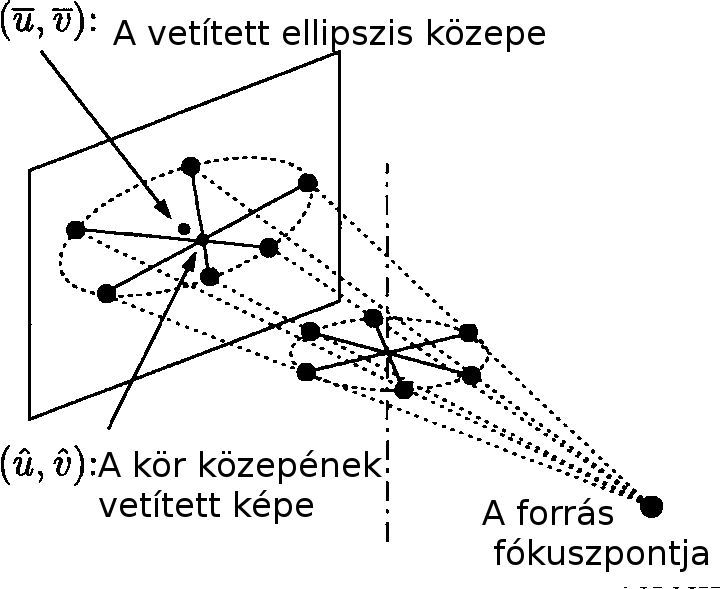
\includegraphics[width=0.5\textwidth]{abrak/etameghat}
\caption{A körbeforduló golyók vetített képe. A forgástengely vetített képe nem feltétlenül esik egybe a vetített ellipszis középpontjával.\cite{noo} }
\label{fig:etameghat}
\end{figure}


\begin{equation}
\label{eq:etameghat1}
\left(u_k^j-u_k^i \right) \hat{v}_k - \left(v_k^j-v_k^i \right) \hat{u}_k = v_k^iu_k^j - v_k^ju_k^i, \hskip10pt  j = i+ \frac{N}{2}, \hskip10pt i = 1 \ldots  \frac{N}{2} 
\end{equation}


\begin{equation}
\label{eq:etameghat2}
\eta = \arctan \left ( \frac{\hat{u}_1 - \hat{u}_2}{\hat{v}_1 - \hat{v}_2} \right )
\end{equation}



Az $\eta$ szög meghatározása után az összes projekción a golyók vetített képeinek koordinátáját el kell forgatni ezzel a szöggel. Ez után a képek úgy kezelhetőek, mintha egy ferdeségtől mentes detektorral készültek volna. Vagyis egy ellipszis ($u_k^i, v_k^i$) pontja helyett \aref({eq:forgatas})~egyenletekkel számolt (${u_k^i}^*, {v_k^i}^*$) pontot vesszük figyelembe a számolás további részében.  Csupán arra kell odafigyelni, hogy a detektoron keresett ($u_0,v_0$) koordinátákat végül vissza kell forgatni .

\begin{equation}
\label{eq:forgatas}
\begin{pmatrix}
{u_k^i}^* \\ {v_k^i}^*
\end{pmatrix}
 = 
 \begin{pmatrix}
 \cos \eta & -\sin \eta \\
 \sin \eta & \cos \eta
\end{pmatrix}
\cdot
\begin{pmatrix}
{u_k^i} \\ {v_k^i}
\end{pmatrix}
\end{equation}


Ez után az elforgatott pontokra ellipszist kell illeszteni, ahol az ellipszis pontjai \aref({eq:ellipse})~egyenletet elégítik ki. 

\begin{equation}
\label{eq:ellipse}
a \left ( {u^i}^* - \overline{u} \right )^2 + b  \left ( {v^i}^* - \overline{v} \right )^2 + 2c  \left ( {u^i}^* - \overline{u} \right ) \left ({v^i}^* - \overline{v} \right ) = 1
\end{equation}


Az fenti egyenletből lineáris regresszióval meghatározhatóak az ellipszis ($\overline{u}, \overline{v}$) középpontjai, az $a$ és $b$ paraméterek, amelyek a tengelyek hosszával vannak kapcsolatban, valamint $c$, amely paraméter az ellipszis ferdeségével hozható összefüggésbe.  Ezekből a paraméterekből először a forrás és a tengely távolsága ($D$) a meghatározható, \aref({eq:noo_d})~egyenletek alapján. Az újonnan meghatározott $D$ távolság ismeretében a további meghatározandó paraméterek \aref({eq:noo_tobbi})~egyenletekkel számolhatóak. Az egyenletekben $z_1$ és $z_2$ a golyók $z$ koordinátájára utal a fantomon. Amennyiben az adott golyó a fantomon a röntgenforrás vonala felett helyezkedik el, úgy előjele pozitív, amennyiben alatta, úgy előjele negatív. Ez az adat sem feltétlenül mérhető, így ezt is az elkészült felvételek alapján kell meghatározni. Továbbá \aref({eq:noo_d}).~egyenletekből az elsőnél látható $\epsilon$ tényező értéke $\pm1$: pozitív előjellel, ha a két golyó a a röntgenforrás két oldalán helyezkedik el, vagyis ha $z_1z_2 < 0$. Amikor a golyók ugyan azon az oldalon vannak, vagyis $z_1z_2>0$, akkor $\epsilon$ értéke lehet $+1$, valamint $-1$ is: ilyen esetben az előjel megállapításához szükséges a felhasználó döntése. Az egyenletekben jelen lévő $n_0, n_1, m_0, m_1, \rho_k, \zeta_k$ változók nem a geometria paraméterei,csupán segédváltozók a többi paraméter számolásához.

\begin{equation}
\label{eq:noo_d}
\left.
\begin{split}
D^2 &= \frac{(a_1- 2n_0n_1 )- \epsilon \sqrt{a_1^2+ 4n_1^2 - 4n_0n_1a_1}}{2n1^2}\\
n_0&= \frac {1-m_0^2-m_1^2}{2m_0m_1}\\
n_1&= \frac{a_2-a_1m_1^2}{2m_0m_1}\\ 
m_0 &=\left ( \overline{v}_2 - \overline{v}_1 \right) \sqrt{b_2-\frac{c_2^2}{a_2}}\\
m_1 &= \sqrt{b_2 - \frac{c_2^2}{a_2}} \sqrt{b_1- \frac{c_1^2}{a_1}} 
\end{split}
\right\}
\end{equation}



\begin{equation}
\label{eq:noo_tobbi}
\left.
\begin{split}
v_0^* &= \overline{v}_1 - \text{sign} (z_1) \frac {\sqrt{a_1 + a_1^2D^2    }}{\sqrt{a_1b_1-c_1^2}}\\
u_0^* &= \frac{1}{2} \overline{u}_1  + \frac{1}{2} \overline{u}_2 + \frac{c_1}{2a_1} \left ( \overline{v}_1 - v_0^* \right) + \frac{c_2}{2a_2} \left (\overline{v}_2 - v_0^* \right)\\
\rho_k &= \frac{\sqrt{a_kb_k-c_k^2}}{\sqrt{a_kb_k+a_k^2b_kD^2-c_k^2}}  \hskip10pt k = 1,2\\
\zeta_k &= D \cdot \text{sign}(z_k)a_k \frac{\sqrt{a_k}}{\sqrt{a_kb_k+a_k^2b_kD^2-c_k^2}}\\
\sin \phi & = -\frac{c_1}{2a_1}  \zeta_1 - \frac{c_2}{2a_2} \zeta_2
\end{split}
\right \}
\end{equation}


Miután a fenti egyenletekkel meghatároztuk a geometriára jellemző $D, v_0^*, u_0^*$ és $\phi$ paramétereket, végül már csak a forrás és forgástengely közötti $R$ távolságot kell meghatároznunk. Ez \aref({eq:noo_r})~egyenlet lapján történik, ahol $d$ a két golyó -- valós -- távolsága a fantomon.

\begin{equation}
\label{eq:noo_r}
\begin{split}
\frac{d^2}{R^2} = \frac{1}{N} \sum_{i=1}^{N} \left\{ \left ( \zeta_1 \frac{u_1^i - u_0^*}{v_1^i - v_0^*}  - \zeta_2 \frac{u_2^i - u_0^*}{v_2^i - v_0^*} \right)^2 + \left( \frac{D \zeta_1}{v_1^i - v_0^*} - \frac{D \zeta_2}{v_2^i - v_0^*} \right)^2 + \left ( \zeta_1 - \zeta_2 \right) ^2 \right\}
\end{split}
\end{equation}


\subsubsection{A paraméterek meghatározása Wu\cite{wu} cikke alapján}


A fentiekhez képest a legnagyobb eltérést az jelenti Noo és Wu cikke között, hogy utóbbi esetben a fantomon nem két golyó van, hanem több, ezzel növelve a módszer megbízhatóságát. 

A paraméterek meghatározása ebben az esetben is az $\eta$ szög meghatározásával és a vele való korrekcióval történik, ám ebben az esetben -- mivel több golyó adata áll rendelkezésre -- egyenes illesztéssel tudjuk meghatározni $\tan \eta$ értékét, \aref({eq:wu_eta})~egyenlet szerint.

\begin{equation}
 \label{eq:wu_eta}
\hat{u}_k  = c + \tan \eta \cdot \hat{v}_k
\end{equation}

A mérési pontokra ez után szintén ellipszist kell illeszteni, azonban Wu cikkében \aref({eq:wu_ellipse})~egyenlet írja le a ellipszist. El van hanyagolva tehát \aref({eq:ellipse})~egyenletben még meglévő $c$ paraméter, amely akkor tehető meg, ha az ellipszis nagytengelye éppen vízszintes állású. Ez jó közelítéssel igaz is, hiszen az ellipszisen el vannak forgatva az előzetesen meghatározott $\eta$ szöggel, amely következtében a forgástengely képe a detektoron egy függőleges egyenes. Mivel az asztal körbeforgatása során a golyók merőlegesen mozognak a forgástengelyre, a vetített képükre is igaz lesz, hogy a pályájuk nagytengelye merőleges a forgástengely vetületére, azaz éppen vízszintes. 

\begin{equation}
\label{eq:wu_ellipse}
a \left ( {u^i}^* - \overline{u} \right )^2 + b  \left ( {v^i}^* - \overline{v} \right )^2  = 1
\end{equation}



Ezzel az egyszerűsítéssel a keresett geometriai paramétereket leíró egyenletek is jócskán leegyszerűsödnek. A keresett $v_0^*$ és $D$ paraméterek  \aref({eq:wu_d})~egyenletekből lineáris regresszióval megkaphatóak, amely egyelnetek a $k$ és $k'$ sorszámú ellipszisek között teremtenek kapcsolatot.

\begin{equation}
\label{eq:wu_d}
\frac{\overline{v}_k + \overline{v}_{k'}}{2}  - \frac{1}{2 \left( \overline{v}_k   - \overline{v}_{k'}  \right)} \left( \frac{1}{b_k} - \frac{1}{b_{k'}} \right) = v_0^* + D^2 \frac{1}{2 \left( \overline{v}_k   - \overline{v}_{k'} \right) }   \left( \frac{a_k}{b_k} - \frac{a_{k'}}{b_{k'}} \right)
\end{equation}

Vegyük észre, hogy Noo módszerével ellentétben itt nem szükséges a golyók függőleges pozíciójának ($z_1, z_2$) vizsgálata. Így ez a módszer minden esetben egyértelműen számolja a kérdéses paramétereket, míg Noo módszerénél az összes többi paraméter értékét meghatározó $D$ paraméter bizonyos esetekben -- amikor a kiválasztott golyók függőlegesen a forrás azonos oldalain voltak -- nem volt egyértelmű. Továbbá ez a képlet jóval egyszerűbb, mint \aref({eq:noo_d})~egyenletekben leírtak.

Ugyancsak egyszerű képletet kapunk $u_0^*$ értékére: mivel a $c$ paraméterek értékét elhanyagoljuk, a Noo által használt (\ref{eq:noo_tobbi}) képletek megfelelő sorára ránézve látszik, hogy $u_0^*$ értéke az ellipszis illesztésnél kapott $\overline{u}_k$ értékek átlagolásával kapható, vagyis  \aref({eq:wu_u0}), ahol $E$ az alkalmazott golyók -- és így az ellipszisek -- száma. 
\begin{equation}
\label{eq:wu_u0}
u_0^* = \frac{1}{E} \sum_{k=1}^E \overline{u}_k\\
\end{equation}


Ez után az egyetlen meghatározandó paraméter a forgástengely és a forrás $R$ távolsága. Ezt a távolságot most \aref({eq:wu_r})~egyenletekkel tudjuk meghatározni, amelyek egy $k$ és egy $k'$ sorszámú ellipszis között teremtenek kapcsolatot, és ahol $d^{kk'}$ a két  ellipszishez tartozó golyók távolsága a fantomon. A képletben továbbá $ \left ( \alpha_k - \alpha_{k'} \right )$ jelöli annak az elfordulásnak a szögét, amely elfordulással a két golyó az ellipszisük azonos fázisába forgathatóak. Ez a szög tehát $0^\circ$, amennyiben a golyók a plexi fantomon a forgástengely azonos oldalára vannak felerősítve, és $180^\circ$, amennyiben a fantom ellentétes oldalain vannak.

\begin{equation}
\label{eq:wu_r}
\left .
\begin{split}
\left( \frac{d^{kk'}}{R} \right) ^2 & = \left ( \zeta_k - \zeta_{k'}  \right )^2  +  \left (\rho_{k} \right )^2 + \left (\rho_{k'} \right )^2  - 2\rho_k \rho_{k'} \cos  \left ( \alpha_k - \alpha_{k'} \right ) \\
\rho_k &= \frac{1}{\sqrt{\left (\overline{v}_k - v_0^* \right)^2 \cdot b_k}}\\
\zeta_k &= \left ( \overline{v}_k  - v_0^* \right ) \frac{ 1- \left( \rho_k \right) ^2 }{D} 
\end{split}
\right\}
\end{equation}


\subsection{A geometriai kalibráló mérés kivitelezése}

A geometriai kalibrációs mérésekhez csapágygolyókat használtunk, amelyeket cellux ragasztóval rögzítettünk egy plexi lapra, \aref{fig:geomfantom}.~ábrán látható módon.


\begin{figure}[htbp]
\center
\includegraphics[width=0.8\textwidth]{abrak/geomfantom}
\caption{A geometriai kalibrációhoz használt fantom}
\label{fig:geomfantom}
\end{figure}


 A plexin 2~mm-enkénti bemélyedés segítette a pontos pozicionálást, a golyókat ezekbe a lyukakba ragasztottuk bele. Továbbá ezen barázdarendszer a golyók távolságának leolvasását is megkönnyítette. A méréseket a lehető legmagasabb csőfeszültség mellett, 80~kV-on végeztük, a fantomot körbeforgatva. A magas feszültségre azért volt szükség, hogy a plexi minél kevésbé legyen látható az elkészült felvételeken, ezzel segítve a golyók megtalálását a képen. Ugyanakkor a magas feszültség ellenére is, amikor a lemez síkja épp párhuzamos volt a fősugárral -- tehát a detektoron \aref{fig:geomfantom}.~ábrán látható elrendezés $90^\circ$-kal való elforgatottja jelent meg, a plexi lemez a fém golyókkal összemérhető intenzitást adott, vagyis a golyók elkülönítése a plexitől ekkor nehezebb feladat, mintha a golyók intenzitása jelentősen eltérni a plexiétől. Egy ilyen helyzetben és egy 90$^\circ$-kal elforgatott helyzetben készült ábrázol \aref{fig:geomfantom_plexi}.~ábra. Láthatjuk rajta, hogy a fősugárra merőleges állásban (a felső képen) a golyók intenzitására 1000--2000 körüli érték adódik, míg a plexinél ez az érték 10~000 körüli. Elforgatott állásban a plexi és a golyók intenzitása is 1000--2000 körüli érték, vagyis ekkor már a plexi elsötétülése megegyezik a golyóékéval. Ez a a jelenség az algoritmusok tervezése során egy megoldandó problémát jelentett, amelyre \aref{sec:kozeppont}.~fejezetben térek ki.






\begin{figure}[htbp]
\center
\includegraphics[width=0.8\textwidth]{abrak/geomfantom_meroleges}
\includegraphics[width=0.8\textwidth]{abrak/geomfantom_parhuzamos}
\caption{A geometriai kalibrációhoz használt fantom}
\label{fig:geomfantom_plexi}
\end{figure}







\subsection{A geometriai kalibráció megvalósítása}



A geometriai kalibráció robusztus algoritmusainak megalkotása során rendelkezésemre állt a kísérleti algoritmus során eredményesnek bizonyult megvalósítás\cite{botond}, ami lényegében \acite{wu} cikken alapult,  valamint felhasználtam  \acite{noo} cikkben leírtakat is. Míg utóbbi csak két golyó adataival dolgozik, kevesebb elhanyagolást alkalmaz. Előbbi azonban egyszerűbb képleteket használ, eleve több golyós fantomot feltételezve, amely gyakran lineáris regresszióvá alakítja a képleteket, felhasználva egyszerre az összes golyó adatait. Mindkét cikk algoritmusát implementáltam a programomban, megvizsgáltam, hogy vajon a kevesebb elhanyagolást eredményező változat robusztussá tehető e, ha a több golyó adatait megfelelő hibaszámítással súlyozva átlagolom. A hibaszámítást a másik algoritmus megvalósítása során is bevezettem, így mindkét módszernél kiküszöbölve az esetleges hibákat a golyók keresése és az ellipszisek illesztése során. Továbbá új algoritmust vezettem be a golyók középpontjának megkeresésére, amely a felhasználótól kevesebb információt kér, pontosabban jár el akkor, amikor a plexi intenzitásban nem tér el eléggé a golyóktól, valamint a videókártyán való megvalósításnak köszönhetően hamar lefut.

A következőkben bemutatom a geometriai korrekciós faktorok meghatározásának folyamatát az elkészült programban, ismertetem a  megtervezett algoritmusokat és azok használatának lehetőségeit és korlátait, valamint az eredményeit.


\subsubsection{ A folyamat áttekintése és a felhasználótól kért adatok. }


Az általam megvalósított kalibrációs szoftver újabb funkciója a geometriai korrekciós mérések kiértékelése. A funkció kiválasztásakor először beolvasásra kerülnek a gain kalibráció adatai, amely helyének kiválasztására a felhasználónak grafikus felületen van lehetősége. Szintén grafikus felületen választható ki az, hogy hol keresse a program a geometriai kalibrációhoz szükséges képkészletet. A mappában lévő képek ezek után egy csúszka mozgatásával átnézhetőek, továbbá szintén grafikus felületen várja a program a szükséges felhasználótól bekérendő adatok megadását. Ezek az adatok a következők:

\begin{itemize}
  \item Első felhasználni kívánt kép.
  \item Azon golyók száma, amelyek az összes képen rajta vannak.
  \item Azon golyók száma, amik nincsenek rajta az összes képen.
  \item Az első képpel azonos állású, $360^\circ$-kal elforgatott kép
  \item A forrás és a detektor becsült távolsága mm-ben.
    \item A fantomon a golyók egymástól vett távolságát.
\end{itemize}

Az első kép kiválasztására azért van lehetőség, mert a felhasználó hibázhat a mérés elindításakor: nem kapcsolja be a röntgen forrást, nem indíja el a motort, stb... A keresendő golyók száma szintén fontos, a golyók keresésénél felhasznált paraméter. Az általam megvalósított algoritmusnak segítséget ad az is, hogy tudja, hogy bizonyos képeken több golyó lehet a képen, mint az elsőn -- például mert a kép alsó és felső szélén lévő golyók vetülete a detektoron kívülre eset és így a képről eltűnhet a forgatás hatására. Ennek megállapításához a felhasználónak eleve át kell néznie azon képeket, amik egy teljes körbefordulás alatt készültek, így arra is megkéri a program, hogy a csúszkát ez után hagyja egy olyan állapotban, amely nagyjából  $360^\circ$-kal van elforgatva az első képhez képest. Itt nem szükséges pontosan a teljes körbeforduláshoz tartozó projekciót megadni, a felhasználó ettől eltérhet $\pm 45^\circ$-kal. A cél itt az, hogy a felhasználó jelölje ki, körül-belül hol kell keresni a teljes körbefordulást, hogy annak megkeresése rövidebb időt vegyen igénybe, mintha az összes projekciót át kellene nézni. Szükséges továbbá a Noo féle számításhoz megadni a detektor és a forrás távolságát. Erre azért van szükség, mert ahogy \aref{sec:noo} fejezetben említettem, a Noo féle módszernél ezen távolság kiszámítása azon esetekben, amikor a két kiszemelt golyó a forgástengely azonos oldalán vannak, nem egyértelmű. Ennek eldöntését segíti a felhasználó által megadott paraméter, amely szintén nagyságrendi becslést kell, hogy adjon, tehát $10~cm$ körüli hiba még megengedett. Ez után egy újabb grafikus felületen kell megadni a fantomon a golyók helyzetét.


Amennyiben ez megtörtént, a felhasználó ellenőrizheti, hogy az algoritmus jó helyen találta e meg a golyókat a kezdeti képen, illetve, hogy a teljes körbefordulás utáni kép egyezik e az elsőnek választottal. Amennyiben bármelyikben hibázott a program, lehetőség van visszalépni, és újabb kezdeti projekciót választani. A grafikus felület egy ilyen állapotát mutatja meg  \aref{fig:geomui}.~ábra. 


\begin{figure}[htbp]
\center
\includegraphics[width=0.8\textwidth]{abrak/geomui}
\caption{A geometriai kalibrációs funkció felhasználói felülete. A felhasználó a fenti mappát választotta ki a képek helyéül. A bal oldali képet választotta első képnek, az alsó részen pedig megadta a szükséges paramétereket. A szoftver meghatározta a teljes körbefordulás utáni projekciót és megkereste a két projekción a gömbök középpontját. }
\label{fig:geomui}
\end{figure}



A kijelölt projekció módosítására egyébként a diplomamunkám elkészítése során nem kellett sort kerítenem, az első képen is biztosan felismerte a golyók helyzetét a program és a körbefordulás utáni képet is stabilan megtalálta. Az esetleges hibás felismerések elkerülése végett ugyanakkor érdemes olyan projekcióról indítani a kalibrációt, amelyen a plexi elsötétedése alacsony mértékű.


A kísérleti algoritmusnál megvalósítottakhoz  képest ez a felület jóval felhasználóbarátabb, kevesebb információt kér a felhasználótól, kisebb a felhasználó hibázási lehetősége is -- ahol a program számot vár, ott szöveget nem tud megadni, stb.

A program a felhasználó jóváhagyása után az alább ismertetett algoritmusokkal kiszámolja a kalibrációs faktorokat, majd az eredményt közli a felhasználóval. A folyamat  jó részét a képek feldolgozása, azaz a golyók középpontjának megkeresése teszi ki. A feldolgozás állapotáról a felhasználó egy folyamatjelző sávon tudja követni.






\subsubsection{Teljes körbefordulás meghatározása}

A szoftver első feladata, még a felhasználótól való adatbekérés során, hogy meghatározza, melyik projekció felel meg az elsőként kiválasztott projekció $360^\circ$-kal való elforgatottjának. Ehhez a felhasználó megad egy viszonyítási alapot: egy olyan képet, amely nagyjából megfelel a fenti kritériumnak. A szoftver ez után a két kép sorszámának különbségét elosztja $8$-cal. A teljes körbefordulás képét a felhasználó által megadott kép körül ilyen távolságban keresi, a képek sorszámainak tekintetében. Így nem kell végignézni a teljes mappa tartalmát és a folyamat felgyorsul. 


A teljes körbefordulást vizsgálatot úgy végzem, hogy az első képpel korrerálom a kiválasztott második képpel, és megvizsgálom, hogy a korreláció melyik képpel a legnagyobb. Ez a kép lesz a teljes körbefordulás utáninak választott kép. A kiválasztott $A$ és $B$ közötti kép $C$ korrelációs együtthatóját \aref({eq:corr})~képlet alapján végzem, ahol az összegzés a kép összes pixelére vonatkozik, a felülvonás az átlagolást jelenti, $\sigma$ pedig a képek szórását jelöli. A műveletet grafikus kártyán, párhuzamosan végzem. Az átlagokat és a szórásokat pedig a művelet előtt, szintén grafikus kártyán párhuzamosítva végzem: az átlagoláshoz a pixelek értékeit össze kell adni, a szórás pedig a pixel értékeinek négyzetösszegéből származtatható. Így valójában mindkét művelet \aref{sec:reduce} fejezetben bemutatott \emph{reduce} műveletet testesíti meg és könnyen párhuzamosítható. 

\begin{equation}
\label{eq:corr}
C = \frac{ \sum_{i=1}^{N}  \left \{ (A_i  - \overline{A} ) \cdot ( B_i - \overline{B} ) \right \} }{N \cdot \sigma_A  \cdot \sigma_B}
\end{equation}


A fenti módon számolt korrelációs érték $0$ és $1$ közötti értéket vehet fel: a kép önmagával való korrelációs együtthatója éppen $1$. Ez alapján a szoftver vizsgálhatja azt is, hogy a megtalált kép eléggé hasonlít e az elsőként kiválasztott képre. Amennyiben a korrelációs együttható $0,\!9$ alatt van, vagyis a két kép nem hasonlít eléggé, a szoftver figyelmezteti a felhasználót.



\subsubsection{A golyók középpontjának meghatározása}
\label{sec:kozeppont}



Amennyiben a felhasználó minden adatot megadott, megkezdődik a képek feldolgozása, amelynek során először meghatározásra kerülnek az egyes projekciókon a golyók koordinátái. Tölgyesi\cite{botond} munkája során erre két algoritmust implementált. Az egyiknél a kép kis részleteinek egy körlap képével való korrelációját számolja. Ez a módszer bizonytalannak bizonyult és ezért már a korábbi munka során el lett vetve. A másik módszere szerint a képeket először invertálja ( hogy a nagy elnyelésű golyók helyén a kép intenzitása nagy legyen), majd golyók helyét a kép egy részletén belül az ott látható képpontok intenzitással súlyozott súlypontjába becsüli.  Ennek az algoritmusnak is van hátulütője. Egyrészt megfelelő méretű ablakot kell választani, hogy a golyó épp beleessen a vizsgált tartományba és ennek az ablaknak a helyét minden projekciónál számon kell tartani. Kifejezetten hibás eredményhez vezethet ez az algoritmus akkor, amikor a golyókat épp a fősugárral párhuzamosan álló plexi lapon próbáljuk megtalálni. Ekkor a plexi lap okozta gyengülés \aref{fig:geomfantom_plexi}.~ábrán látottak alapján összemérhető, vagy akár nagyobb, mint a golyó által okozott. A plexi ilyenkor jelentős mértékben befolyásolni tudja a súlypontkeresést, akár téves útra térítve a golyók keresését. Ez ellen a vizsgált ablak csökkentésével lehet, de teljesen nem kiküszöbölhető.

A fenti hibák elkerülése érdekében a körök középpontjainak megkereséséhez egy új fajta  algoritmust használtam fel: a Hough-transzformációt. Ez az igen széles körben használt módszer  körök, egyenesek, illetve akár tetszőleges alakzatok lokalizálására használható. Körök keresése esetében először a képeken található éleket kell megkeresni, vagyis a képen található körök szélén lévő pixeleket. Ez után a megtalált él-pixelekből kell köröket rajzolni. \Aref{fig:houghcircles}.~ábrán is szemléltetett módon a szélekből rajzolt körök épp 




\begin{figure}[htbp]
\center
\includegraphics[width=0.6\textwidth]{abrak/houghcircles}
\caption{Körkeresés Hough-transzformációval.}
\label{fig:geomfantom_plexi}
\end{figure}




\begin{table}[]
\centering
\label{tab:logkernel}
\begin{tabular}{|c|c|c|c|c|c|c|c|c|}
\hline
0.0046  & 0.0034  & 0.0013  & -0.0008 & -0.0016 & -0.0008 & 0.0013  & 0.0034  & 0.0046  \\ \hline
0.0034  & 0       & -0.0048 & -0.009  & -0.0107 & -0.009  & -0.0048 & 0       & 0.0034  \\ \hline
0.0013  & -0.0048 & -0.0126 & -0.0193 & -0.022  & -0.0193 & -0.0126 & -0.0048 & 0.0013  \\ \hline
-0.0008 & -0.009  & -0.0193 & -0.0281 & -0.0316 & -0.0281 & -0.0193 & -0.009  & -0.0008 \\ \hline
-0.0016 & -0.0107 & -0.022  & -0.0316 & -0.0354 & -0.0316 & -0.022  & -0.0107 & -0.0016 \\ \hline 
-0.0008 & -0.009  & -0.0193 & -0.0281 & -0.0316 & -0.0281 & -0.0193 & -0.009  & -0.0008 \\ \hline
0.0013  & -0.0048 & -0.0126 & -0.0193 & -0.022  & -0.0193 & -0.0126 & -0.0048 & 0.0013  \\ \hline
0.0034  & 0       & -0.0048 & -0.009  & -0.0107 & -0.009  & -0.0048 & 0       & 0.0034  \\ \hline
0.0046  & 0.0034  & 0.0013  & -0.0008 & -0.0016 & -0.0008 & 0.0013  & 0.0034  & 0.0046  \\\hline
\end{tabular}
\caption{ $\sigma$  = 1.4 paraméterű Gauss függvény Laplace-transzformáltja.  }
\end{table}




\clearpage

%\begin{thebibliography}{9}

\bibliographystyle{abbrv}
\bibliography{bibfile} 


%
%\bibitem{reduce}
%Mark Harris,
%{\it Optimizing Parallel Reduction in CUDA},
%{\tt online: http://docs.nvidia.com/cuda/samples/6\_Advanced/reduction/doc/reduction.pdf},
%Utolsó hozzáférés: 2016.05.28. 14:00
%
%\bibitem{Noo}
%Frédéric Noo, Rolf Clackdoyle, Catherine Mennessier, Timothy A White, Timothy J Roney,
% {,,Analytic method based on identification of ellipse parameters for scanner calibration in cone-beam tomography},
% \emph{Physics in Medicine and Biology},
% vol. 45,
%  number={11},
%  pages={3489},
%  url={http://stacks.iop.org/0031-9155/45/i=11/a=327},
%  year={2000},
%  abstract={This paper is about calibration of cone-beam (CB) scanners for both x-ray computed tomography and single-photon emission computed tomography. Scanner calibration refers here to the estimation of a set of parameters which fully describe the geometry of data acquisition. Such parameters are needed for the tomographic reconstruction step. The discussion is limited to the usual case where the cone vertex and planar detector move along a circular path relative to the object. It is also assumed that the detector does not have spatial distortions. We propose a new method which requires a small set of measurements of a simple calibration object consisting of two spherical objects, that can be considered as `point' objects. This object traces two ellipses on the detector and from the parametric description of these ellipses, the calibration geometry can be determined analytically using explicit formulae. The method is robust and easy to implement. However, it is not fully general as it is assumed that the detector is parallel to the rotation axis of the scanner. Implementation details are given for an experimental x-ray CB scanner.}
%}
	
%\bibitem{url}
%{\tt http://fizipedia.bme.hu/index.php/Gamma\_spektroszkópia},
%2013.~november~29., 1:00

%\bibitem {nagy}
%Nagy L. Gy.,
%{\it Radiokémia és izotóptechnika},
%Tankönyvkiadó, Budapest, 1983.
%\bibitem {lederer}
%C.M. Lederer, J.M. Hollander, I. Perlman,
%{\it \foreignlanguage{english}{Table of Isotopes}},
%Wiley, New York, 1984.
%\end{thebibliography}
\end{document}